% !TeX encoding = UTF-8
% !TeX program = xelatex
% !TeX spellcheck = fr_CA
\documentclass[nuit,charter,pied,handout]{BeamerJS}
\title{Introduction aux probabilités discrètes}
\subtitle{À l'intention des étudiants de STT-1500}
\institute{Université Laval}
\fonction{Département de mathématiques et de statistique}
\logotitre{../logo_UL.pdf}
\author{Jérôme Soucy}
\date{Hiver 2025}

\usepackage{commandesJS}
\addbibresource{../references.bib}
\NouvelleBoiteJS{defns}{Définitions}{Dominante}{DominanteBG}
\NouvelleBoiteJS{props}{Propositions}{VertPreuve}{PreuveBG}
\NouvelleBoiteJS{exs}{Exemples}{GrisExemple}{ExempleBG}
\NouvelleBoiteJS{rems}{Remarques}{Accent}{AccentBG}
\usepackage{adjustbox}

% Encadré sans titre (remplace l'ancienne boite)
\newtcolorbox{cadre}{enhanced, breakable, sharp corners, boxrule=0.7pt,
	colback=Fond, colframe=Dominante!45, top=8pt, bottom=8pt,
	left=10pt, right=10pt, before skip=10pt, after skip=8pt}

\begin{document}
\begin{frame}[plain,noframenumbering]
	\titlepage
\end{frame}
\begin{frame}{Résumé}
\tableofcontents
\end{frame}	
\section{Origines}
\begin{frame}{Le problème de Galilée}
	\pause
	\begin{cadre}
		On a observé que bien que \num{9} et \num{10} puissent être obtenus comme totaux de trois dés de \num{6} manières différentes, la somme de \num{9} est obtenue moins souvent que la somme de \num{10}. Pourquoi?
	\end{cadre}
	\pause
	\centering\begin{adjustbox}{center, width=.9\textwidth}
		{\small\begin{tabular}{|
				>{\columncolor{Dominante}}l |l|l|l|l|l|l|}
			\hline
			\color{white}{Somme de $9$}  & $6+2+1$ & $5+3+1$ & $5+2+2$ & $4+4+1$ & $4+3+2$ & $3+3+3$ \\ \hline
			\color{white}{Somme de $10$} & $6+3+1$ & $6+2+2$ & $5+4+1$ & $5+3+2$ & $4+4+2$ & $4+3+3$ \\ \hline
		\end{tabular}}
	\end{adjustbox}
	\hfill
	\pause 
	\begin{lumiere}
		Pour la première fois, l'expérience du hasard fait appel à la théorie pour obtenir des explications. \cite{picard}
	\end{lumiere}
\end{frame}

\begin{frame}[c]{Hasard?}
\pause 
	Galilée est mort le 8 janvier 1642, année de naissance de Newton. Trois cents ans plus tard --- jour pour jour ---, Stephen Hawking naissait.
	\pause 
	\vfill
	\hfill
	\begin{minipage}[c]{.4\textwidth}
		\centering 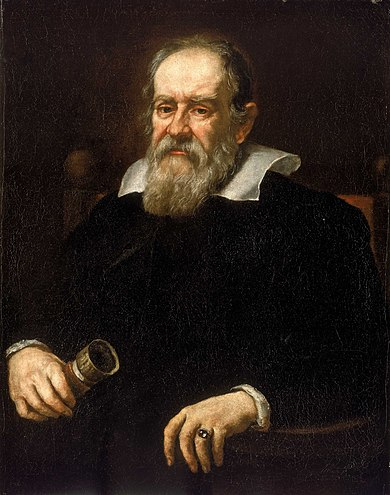
\includegraphics[height=5cm]{images/Galilee}\\
		\centering Galilée (1564-1642)
	\end{minipage} 
	\pause 
	\hfill
	\begin{minipage}[c]{.4\textwidth}
		\centering 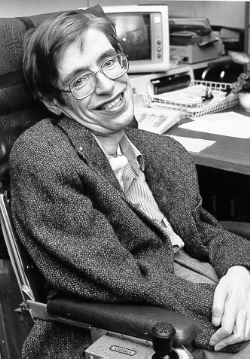
\includegraphics[height=5cm]{images/Hawking}\\
		\centering Stephen Hawking (1942-2018)
	\end{minipage}
	\hfill
\end{frame}


\begin{frame}[c]{Le problème des partis}
\pause 
	Le chevalier de Méré, de son vrai nom Antoine Gombaud (1607-1684), tint une correspondance avec Blaise Pascal (1623-1662) sur un problème lié à la répartition des gains (ou pertes) lorsqu'un jeu de hasard est interrompu.
	\pause 
	\begin{cadre}
		Deux joueurs jouent à un jeu de hasard. Ils ont chacun misé un montant $m$ au départ. Celui qui remportera la cagnotte (dont le montant est $2m$) sera celui à avoir gagné le premier 3 parties (pas nécessairement consécutives). Or il se trouve que le jeu est interrompu avant que l'un des deux joueurs ait obtenu 3 victoires. Comment, dans ces circonstances, doit-on partager les enjeux ?
	\end{cadre}
\end{frame}

\begin{frame}{L'été 1654}
	\pause 
	\hfill
	\begin{minipage}[c]{.4\textwidth}
		\centering 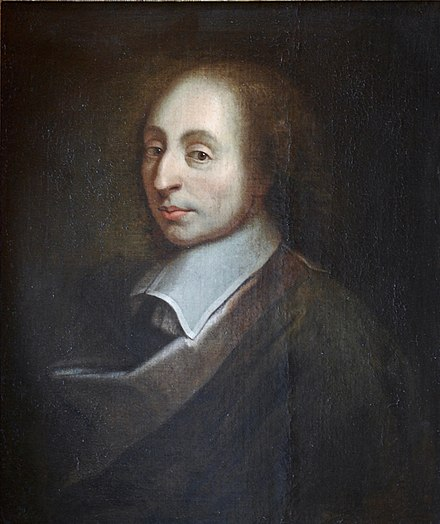
\includegraphics[height=6cm]{images/Pascal}\\
		\centering Blaise Pascal (1623-1662)
	\end{minipage} 
	\hfill \pause 
	\begin{minipage}[c]{.4\textwidth}
		\centering 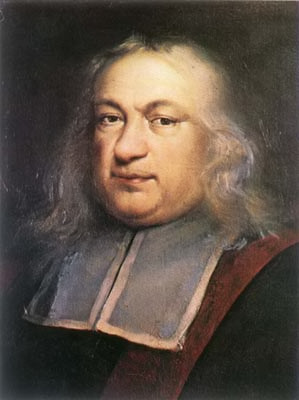
\includegraphics[height=6cm]{images/Fermat}\\
		\centering Pierre de Fermat (1607-1665)
	\end{minipage}
	\hfill
\end{frame}

\section{Expériences aléatoires et événements}
\begin{frame}[c]{Expérience aléatoire}
\pause 
	\begin{defn}
		Une \defi{expérience aléatoire} est une expérience satisfaisant les caractéristiques suivantes\,:
		\begin{enumerate}
			\item elle peut être répétée un grand nombre de fois;
			\item dans des conditions identiques;
			\item on ne doit pas pouvoir prédire avec exactitude son résultat.
		\end{enumerate}
	\end{defn}
\pause
\begin{rem}
La troisième condition est équivalente à affirmer que des résultats différents peuvent être observés même si les conditions 1 et 2 sont satisfaites.
\end{rem}
\end{frame}

\begin{frame}[t]{L'espace fondamental ou l'univers des possibles}\pause 
	\begin{defn}
		Le résultat d'une expérience aléatoire s'appelle un \defi{événement élémentaire} ou encore une \defi{éventualité}.
	\end{defn}\pause 
	\begin{defn}
		L'ensemble dont les éléments sont les événements élémentaires d'une expérience aléatoire s'appelle l'\defi{espace fondamental} ou encore l'\defi{univers des possibles}.
	\end{defn}
	\end{frame}
	\begin{frame}{Notation}
	\pause
	\begin{rem}
	Étant donnée une expérience aléatoire $\mathcal{E}$, un événement élémentaire type s'écrit souvent à l'aide de la lettre grecque omega minuscule $\omega$. \pause Son espace fondamental est généralement représenté à l'aide de la lettre grecque omega majuscule $\Omega$.
	\end{rem}
\end{frame}

\begin{frame}{Exemple : Lancer d'une pièce de monnaie}
	Lorsqu'on lance une pièce de monnaie, \textit{pile} et \textit{face} sont les événements élémentaires. On peut les noter simplement par les lettres $P$ et $F$. Ainsi, $\{P,F\}$ constitue l'espace fondamental. On peut aussi convenir de noter \textit{pile} par un $0$ et \textit{face} par un $1$, auquel cas l'espace fondamental serait donné par $\{0,1\}$.
	
	\pause 
	\begin{lumiere}
		Utiliser des nombres ou des couples de nombres est une bonne pratique pour décrire les éventualités d'une expérience aléatoire. L'utilisation de lettres est aussi appropriée. L'important est de pouvoir facilement comprendre le symbolisme associé à tous les événements élémentaires de l'espace fondamental.
	\end{lumiere}
\end{frame}

\begin{frame}[t]{Les événements en probabilités}\pause 
	Considérons une expérience aléatoire d'espace fondamental $\Omega$. On s'intéresse au cas où le résultat de l'expérience aléatoire figure dans un sous-ensemble déterminé a priori.\pause 
	\begin{defn}
		Soit $\Omega$ l'espace fondamental d'une expérience aléatoire. Un sous-ensemble de $\Omega$ est alors appelé un \defi{événement}.
	\end{defn}
\end{frame}

\begin{frame}[t]{Les événements en probabilités (suite)}
\begin{defns}
	Soit $\Omega$ l'espace fondamental d'une expérience aléatoire. Soit $A$ un sous-ensemble de $\Omega$. 
	\begin{itemize}
	\item Si $A\neq\emptyset$, on dira que $A$ est un \defi{événement possible}. 
	\item Dans le cas contraire, on dira que $A$ est un \defi{événement impossible}. 
	\item Si $A=\Omega$, on dira que $A$ est un \defi{événement certain}.
	\end{itemize}
\end{defns}
\end{frame}

\begin{frame}{Exemple : Trois lancers d'une pièce de monnaie}
	On lance une pièce de monnaie \num{3} fois. On représente \textit{pile} par $P$ et \textit{face} par $F$. Décrivez $\Omega$.\\[0.3cm] \pause 
	On définit les événements suivants : \pause 
	\begin{itemize}
		\item[{\color{black}\(A=\)}] Le nombre d'occurrences de pile est strictement supérieur au nombre d'occurrences de face\,; 
		\item[{\color{black}\(B=\)}] Le nombre d'occurrences de face est strictement supérieur au nombre d'occurrences de pile\,; 
		\item[{\color{black}\(C=\)}] Le nombre d'occurrences de pile est égal au nombre d'occurrences de face.
	\end{itemize}
	\pause
	Décrivez les éventualités appartenant à chacun de ces événements.
\end{frame}

\section{Opérations sur les événements}

\begin{frame}[c]{Pourquoi des opérations sur les événements?}
\pause
\begin{itemize}
	\item Les événements sont des ensembles (sous-ensembles de \(\Omega\)).\pause
	\item On doit pouvoir combiner des événements pour en créer de nouveaux.\pause
	\item Les opérations ensemblistes (union, intersection, complémentaire) ont une interprétation probabiliste naturelle.
\end{itemize}
\end{frame}

\begin{frame}[t]{Événements mutuellement exclusifs (incompatibles)}
\pause
 Voici une représentation où les ensembles $A$ et $B$ (sous-ensembles d'un ensemble $\Omega$) sont disjoints, c'est-à-dire qu'ils ne partagent aucun élément.\\[0.5cm]
 \pause
 \begin{columns}[c]
	\begin{column}{0.5\textwidth}
		\begin{tikzpicture}
			\node[draw,
			circle,
			minimum size =2cm,
			color=Dominante,
			fill=Dominante!40,
			label={[label distance=0.25cm,font=\large, color=Dominante]45:$A$}] (circle1) at (0,0){};

			\node[draw,
			circle,
			minimum size =2cm,
			fill=Accent!50,
			color=Dominante,
			label={[label distance=0.25cm,font=\large,color=Dominante]45:$B$}] (circle2) at (3,0){};
			\draw (-1.5,-1.5) node[below]{$\Omega$} -- (4.5,-1.5) -- (4.5,1.5) -- (-1.5,1.5) -- cycle;
		\end{tikzpicture}
		\[A\cap B=\emptyset\]
	\end{column}
	\pause
 	\begin{column}{0.5\textwidth}
 		En termes probabilistes, on peut voir $A$ et $B$ comme des événements pouvant être définis dans le contexte d'une expérience aléatoire \(\mathcal{E}\) dont l'espace fondamental est $\Omega$. Si les ensemble $A$ et $B$ sont disjoints, on dit que $A$ et $B$ sont des \textbf{événements mutuellement exclusifs} ou encore \textbf{incompatibles}.
 	\end{column}
 \end{columns}
\end{frame}
\begin{frame}[c]{Intersection de deux ensembles}
\pause
	\begin{columns}[c]
		\begin{column}{0.5\textwidth}
			\begin{tikzpicture}[thick,
    							set/.style = {circle,
        						minimum size = 3.6cm,
        						fill=Dominante!40}]
        		\draw[fill=Dominante!5] (-2,-2) node[below]{$\Omega$} -- (4.5,-2) -- (4.5,2) -- (-2,2) -- cycle;
				% Set A
				\node[set,label={135:$A$}] (A) at (0,0) {};
 
				% Set B
				\node[set,label={45:$B$}] (B) at (1.8,0) {};
				 
				% Intersection
				\begin{scope}
				    \clip (0,0) circle(1.8cm);
				    \clip (1.8,0) circle(1.8cm);
				    \fill[Accent](0,0) circle(1.8cm);
				\end{scope}
				 
				% Circles outline
				\draw (0,0) circle(1.8cm);
				\draw (1.8,0) circle(1.8cm);
				 
				% Set intersection label
				\node at (0.9,0) {$A\cap B$};
				
			\end{tikzpicture}
		\end{column}
		\pause
		\begin{column}{0.5\textwidth}
			En termes probabilistes, Si \(A\) et \(B\) sont des événements pouvant être définis dans le contexte d'une expérience aléatoire $\mathcal{E}$, l'\textbf{intersection} de \(A\) et \(B\) correspond à l'événement dont les éventualités appartiennent à \(A\) \textbf{et} à \(B\). Si cette intersection est non-vide, on dit que \(A\) et \(B\) sont \textbf{compatibles}.
		\end{column}
	\end{columns}
\end{frame}
\begin{frame}{Exemple : Trois lancers et l'incompatibilité}
	On lance une pièce de monnaie \num{3} fois. Nous avons vu que \(\Omega\) correspond à
	\begin{align*}
	\{&(P,P,P),(P,P,F),(P,F,P),(F,P,P),\\
	  &(F,F,P),(F,P,F),(P,F,F),(F,F,F)\}.
	\end{align*}
	\pause
	On définit les événements suivants :
	\begin{itemize}
		\item[\color{black}\(A=\)] Le nombre d'occurrences de pile est strictement supérieur au nombre d'occurrences de face; 
		\item[\color{black}\(B=\)] Le nombre d'occurrences de face est strictement supérieur au nombre d'occurrences de pile; 
		\item[\color{black}\(D=\)] Le nombre d'occurrences de pile est de \num{2}. 
	\end{itemize}
	\pause
	Parmi ces événements, identifiez les paires d'événements incompatibles et les paires d'événements compatibles.
\end{frame}
\begin{frame}[c]{Union de deux ensembles}\pause
	\begin{columns}[c]
		\begin{column}{0.5\textwidth}
			\begin{tikzpicture}
				% Set A
				\node [circle,
				    fill=Dominante!40,
				    minimum size =3cm,
				    label={135:$A$}] (A) at (0,0){};
				 
				% Set B
				\node [circle,
				    fill=Dominante!40,
				    minimum size =3cm,
				    label={45:$B$}] (B) at (1.8,0){};
				 
				% Circles outline
				\draw[Accent,thick] (0,0) circle(1.5cm);
				\draw[Accent,thick] (1.8,0) circle(1.5cm);
				 
				% Union text label
				\node[black] at (0.9,-1.8) {$A\cup B$}; 
				\end{tikzpicture}
		\end{column}
		\pause
		\begin{column}{0.5\textwidth}
			En termes probabilistes, Si \(A\) et \(B\) sont des événements pouvant être définis dans le contexte d'une expérience aléatoire $\mathcal{E}$, l'\textbf{union} de \(A\) et \(B\) correspond à l'événement dont les éventualités appartiennent à \(A\) \textbf{ou} à \(B\).
		\end{column}
	\end{columns}
\end{frame}


\begin{frame}[t]{La différence de deux ensembles}
\pause
	\begin{columns}[c]
		\begin{column}{0.5\textwidth}
			\begin{tikzpicture}[thick,
			    set/.style = { circle, minimum size = 3cm}]
			 
				% Set A
				\node[set,fill=Dominante!40,label={135:$A$}] (A) at (0,0) {};
				 
				% Set B
				\node[set,fill=Accent,label={45:$B$}] (B) at (0:2) {};
				 
				% Circles outline
				\draw (0,0) circle(1.5cm);
				\draw (2,0) circle(1.5cm);
				 
				% Difference text label
				\node[left] at (A.center){{\color{white}\(A\setminus B\)}};
			 
			\end{tikzpicture}
		\end{column}
		\pause
		\begin{column}{0.5\textwidth}
			En termes probabilistes, Si \(A\) et \(B\) sont des événements pouvant être définis dans le contexte d'une expérience aléatoire $\mathcal{E}$, la \textbf{différence} de \(A\) et \(B\) correspond à l'événement dont les éventualités appartiennent à \(A\) \textbf{mais pas} à \(B\).
		\end{column}
	\end{columns}
	\pause
	\begin{lumiere}
		La différence de \(A\) et \(B\) n'est pas la même chose que la différence de \(B\) et \(A\). Dans le premier cas, elle correspond à l'ensemble \(A\setminus B\) alors que dans le second elle correspond à l'ensemble \(B\setminus A\).
	\end{lumiere}
\end{frame}
\begin{frame}[c]{L'événement complémentaire}
\pause
	\begin{columns}[c]
		\begin{column}{0.5\textwidth}
			\begin{tikzpicture}
				\draw[fill=Dominante!5] (-1.5,-1.5) node[below]{$\Omega$} -- (4.5,-1.5) -- (4.5,1.5) -- (-1.5,1.5) -- cycle;
				% Circle with label distance 0.5cm
				\node[draw,
				circle,
				color=Dominante,
				minimum size =2cm,
				fill=Dominante!40,
				label={[label distance=-1.5cm,font=\large, color=white]45:$A$}] (circle1) at (0,0){};
				\draw (3,0) node{$A\comp$};
				
			\end{tikzpicture}
			\[A\comp=\Omega\setminus A\]
		\end{column}
		\begin{column}{0.5\textwidth}
			En termes probabilistes, Si $A$ est un événement pouvant être défini dans le contexte d'une expérience aléatoire $\mathcal{E}$, l'\textbf{événement complémentaire} de $A$ correspond à l'ensemble des événements élémentaires de l'espace fondamental qui ne correspondent pas à une réalisation de $A$. On le note $A\comp$. On dira aussi que $A$ et $A\comp$ sont complémentaires.
		\end{column}
	\end{columns}
	\pause
	\begin{lumiere}
		Avec cette notion, on peut observer que \(A\setminus B=A\cap B\comp\).
	\end{lumiere}
\end{frame}
\begin{frame}[t]{Sous-ensembles}
\pause
	\begin{columns}[c]
		\begin{column}{0.5\textwidth}
			\centering\begin{tikzpicture}[thick,
    set/.style = {circle,
        minimum size = 3cm,
        fill=Dominante!40}]
				% Set A
				\node[set,label={135:$A$},color=Dominante] (A) at (0,0) {};
 
				\draw[fill=Accent,color=Accent] (0.5,0.5) circle (0.5cm);
				\node[label={135:{\color{Accent}$B$}},minimum size=0.65cm] at (0.5,0.5) {};
			\end{tikzpicture}
			\[B\subseteq A\]
		\end{column}
		\pause
		\begin{column}{0.5\textwidth}
			En termes probabilistes, Si \(A\) et \(B\) sont des événements pouvant être définis dans le contexte d'une expérience aléatoire $\mathcal{E}$, affirmer que la réalisation de \(B\) implique la réalisation de \(A\) signifie que \(B\subseteq A\).
		\end{column}
	\end{columns}
\end{frame}

\begin{frame}[t]{Récapitulatif des opérations ensemblistes}
\pause
\begin{center}
{\small
\begin{tabular}{|l|l|l|}
\hline
\textbf{Opération} & \textbf{Notation} & \textbf{Interprétation probabiliste} \\ \hline
Intersection & \(A\cap B\) & \(A\) \textbf{et} \(B\) se réalisent \\ \hline
Union & \(A\cup B\) & \(A\) \textbf{ou} \(B\) se réalise \\ \hline
Différence & \(A\setminus B\) & \(A\) se réalise \textbf{mais pas} \(B\) \\ \hline
Complémentaire & \(A\comp\) & \(A\) \textbf{ne se réalise pas} \\ \hline
Inclusion & \(B\subseteq A\) & Si \(B\) se réalise, alors \(A\) aussi \\ \hline
Disjoints & \(A\cap B=\emptyset\) & \(A\) et \(B\) sont incompatibles \\ \hline
\end{tabular}
}
\end{center}
\pause
\vfill
\begin{lumiere}
Relations utiles : \(A\setminus B = A\cap B\comp, A\comp\cap B\comp = (A\cup B)\comp\) et \(\comp{A\cap B}=A\comp\cup B\comp\)
\end{lumiere}
\end{frame}

\begin{frame}{Exemple : Trois lancers --- suite}
	\vspace{-0.5cm}
\begin{itemize}
	\item[\color{black}\(A=\)] Le nombre d'occurrences de pile est strictement supérieur au nombre d'occurrences de face; 
	\item[\color{black}\(B=\)] Le nombre d'occurrences de face est strictement supérieur au nombre d'occurrences de pile; 
	\item[\color{black}\(E=\)] Le nombre d'occurrences de pile est \(\geq 1\).\pause
\end{itemize}
\begin{cadre}
\begin{enumerate}
	\item Parmi les événements \(A, B\) et \(E\), pouvez-vous en trouver qui sont complémentaires? 
	\item Est-ce qu'un de ces événements se réalise dès qu'un autre se réalise? 
	\item Est-ce que \(B\setminus E = B\)?
	\item Est-ce que \(A\setminus E = A\)?
\end{enumerate}
\end{cadre}
\end{frame}

%%%%%%%%%%%%%%%%%%%%%%

\section{Probabilités sur un espace discret}

\begin{frame}[t]{Espace fondamental discret}
\pause
	\begin{defn}
		On dit que l'espace fondamental \(\Omega\) d'une expérience aléatoire est \defi{discret} s'il est fini ou infini dénombrable, c'est-à-dire si on peut énumérer ses éléments sous la forme
		\[\Omega=\{\omega_1,\omega_2,\ldots,\omega_n\}\qquad\text{ou}\qquad\Omega=\{\omega_1,\omega_2,\omega_3,\ldots\}.\]
	\end{defn}
	\pause
	\begin{exs}
		Lancer un dé : \(\Omega=\{1,2,\ldots,6\}\) est fini. \pause Lancer une pièce jusqu'à l'obtention de pile et noter le nombre de lancers : \(\Omega=\Ns\) est infini dénombrable.
	\end{exs}
	\pause
	\begin{lumiere}
		Dans ce module, tous les espaces fondamentaux sont discrets.
	\end{lumiere}
\end{frame}

\begin{frame}[t]{Une loi de probabilité sur un espace discret}
\pause
	\begin{defn}
		Soit \(\Omega\) un espace fondamental discret. Une \defi{loi de probabilité} sur \(\Omega\) est la donnée, pour chaque éventualité \(\omega\in\Omega\), d'un nombre \(p(\omega)\), appelé le \defi{poids} de \(\omega\), tel que\pause
		\begin{enumerate}
			\item \(p(\omega)\geq 0\) pour tout \(\omega\in\Omega\);\pause
			\item \(\displaystyle\sum_{\omega\in\Omega}p(\omega)=1\).
		\end{enumerate}
		\pause
		La \defi{probabilité} d'un événement \(A\subseteq\Omega\) est alors définie par
		\[\P{A}=\sum_{\omega\in A}p(\omega).\]
	\end{defn}
\end{frame}

\begin{frame}{Remarques sur la définition}
\pause
	\begin{rems}
		\begin{itemize}
			\item En particulier, \(\P{\{\omega\}}=p(\omega)\) : le poids d'une éventualité est la probabilité de l'événement élémentaire correspondant.\pause
			\item Comme les termes sont positifs, l'ordre dans lequel on fait la somme n'a pas d'importance, même lorsque \(A\) est infini.\pause
			\item Choisir une loi de probabilité, c'est \emph{modéliser} l'expérience : le cadre mathématique ne dit pas quels poids sont les bons, seulement quelles règles ils doivent respecter.
		\end{itemize}
	\end{rems}
\end{frame}

\begin{frame}{Exemple : Un dé truqué}
\pause
	Un dé est truqué de sorte que la face \(6\) sort une fois sur deux et que les autres faces sont équiprobables.
	\pause
	\begin{center}
	\begin{tabular}{|c|c|c|c|c|c|c|}
		\hline
		\(\omega\) & \(1\) & \(2\) & \(3\) & \(4\) & \(5\) & \(6\) \\ \hline
		\(p(\omega)\) & \(\frac{1}{10}\) & \(\frac{1}{10}\) & \(\frac{1}{10}\) & \(\frac{1}{10}\) & \(\frac{1}{10}\) & \(\frac{1}{2}\) \\ \hline
	\end{tabular}
	\end{center}
	\pause
	\begin{cadre}
		Vérifiez qu'il s'agit bien d'une loi de probabilité. Calculez ensuite la probabilité d'obtenir un nombre pair.
	\end{cadre}
	\pause
	{\color{Dominante}Réponse : \(\P{\{2,4,6\}}=\frac{1}{10}+\frac{1}{10}+\frac{1}{2}=\frac{7}{10}\).}
\end{frame}

\begin{frame}[t]{Premières propriétés}
\pause
	\begin{prop}
		Soit \(p\) une loi de probabilité sur un espace fondamental discret \(\Omega\). Alors
		\begin{enumerate}
			\item \(\P{\emptyset}=0\), \(\P{\Omega}=1\) et \(0\leq\P{A}\leq 1\) pour tout événement \(A\);\pause
			\item \textbf{(Additivité)} si \(A\) et \(B\) sont incompatibles, alors
			\[\P{A\cup B}=\P{A}+\P{B}.\]
		\end{enumerate}
	\end{prop}
	\pause
	Pour l'additivité : chaque éventualité de \(A\cup B\) appartient à un seul des deux événements. Ainsi
	\[\P{A\cup B}=\sum_{\omega\in A\cup B}p(\omega)=\sum_{\omega\in A}p(\omega)+\sum_{\omega\in B}p(\omega)=\P{A}+\P{B}.\]
\end{frame}

\begin{frame}[t]{Additivité pour une famille d'événements}
\pause
	\begin{prop}
		Soit \(A_1,A_2,\ldots\) des événements deux à deux incompatibles d'un espace fondamental discret. Alors
		\[\P{\bigcup_{k=1}^{\infty}A_k}=\sum_{k=1}^{\infty}\P{A_k}\]
		(et de même pour une famille finie).
	\end{prop}
	\pause
	On regroupe les poids selon l'unique \(A_k\) contenant chaque éventualité.
	\pause
	\begin{lumiere}
		Ces règles deviendront les axiomes de Kolmogorov (module \emph{Fondements}).
	\end{lumiere}
\end{frame}

\begin{frame}[t]{Le cas équiprobable où \(\card{\Omega}< \infty\)}
\pause
	\begin{prop}{}{}
		Soit $n\in\Ns$ et soit $\Omega=\{\omega_1,\omega_2,\ldots, \omega_n\}$ l'espace fondamental d'une expérience aléatoire où les éventualités sont équiprobables. Alors
		\[p(\omega_i)=\P{\{\omega_i\}}=\frac{1}{n}\qquad\forall i\in\{1,2,\ldots,n\}.\]
	\end{prop}
	\pause
	Soit \(p\) la valeur commune des poids \(p(\omega_i)\). Puisque la somme des poids vaut \(1\),
	\[1=\sum_{k=1}^n p(\omega_k)=\sum_{k=1}^n p=n\cdot p,\qquad\text{d'où}\qquad p=\frac{1}{n}.\]
\end{frame}
\begin{frame}[t]{Le cas équiprobable où \(\card{\Omega}< \infty\) --- suite}
	\pause
	\begin{prop}{}{}
		Soit une expérience aléatoire \(\mathcal{E}\) d'espace fondamental fini \(\Omega\) dont les éventualités sont équiprobables. Alors, pour tout événement \(A\),
		\[\P{A}=\sum_{\omega\in A}\frac{1}{\card{\Omega}}=\frac{\card{A}}{\card{\Omega}}.\]
	\end{prop}
	\pause
	\begin{lumiere}
		Calculer une probabilité revient alors à \emph{compter} : c'est l'objet du module sur le dénombrement.
	\end{lumiere}
	\pause
	\begin{rem}
		Un espace infini dénombrable ne peut pas être équiprobable : la somme \(\sum_{k=1}^{\infty}p\) vaut \(0\) ou \(\infty\), jamais \(1\).
	\end{rem}
\end{frame}
\begin{frame}{Exemple : Retour sur le problème de Galilée}
	\centering\begin{adjustbox}{center, width=.9\textwidth}
		{\small\begin{tabular}{|
				>{\columncolor{Dominante}}l |l|l|l|l|l|l|}
			\hline
			\color{white}{Somme de $9$}  & $6+2+1$ & $5+3+1$ & $5+2+2$ & $4+4+1$ & $4+3+2$ & $3+3+3$ \\ \hline
			\color{white}{Somme de $10$} & $6+3+1$ & $6+2+2$ & $5+4+1$ & $5+3+2$ & $4+4+2$ & $4+3+3$ \\ \hline
		\end{tabular}}
	\end{adjustbox}
	\pause
	\begin{cadre}
	Calculez la probabilité de réalisation de chacun des ces événements.
	\end{cadre}
\end{frame}

\begin{frame}{Exemple : Retour sur le problème des partis}
	Deux joueurs jouent à un jeu de hasard. Ils ont chacun misé un montant $m$ au départ. Celui qui remportera la cagnotte (dont le montant est $2m$) sera celui à avoir gagné le premier 3 parties (pas nécessairement consécutives). Or il se trouve que le jeu est interrompu après que le joueur 1 ait gagné une partie et le joueur 2 aucune.
	\pause
	\begin{cadre}
	Si le jeu s'était poursuivi, quelle aurait été la probabilité de gain pour chacun des joueurs?
	\end{cadre}
\end{frame}

\begin{frame}{Exemple : Solution du problème des partis}
Le joueur 1 a besoin de 2 victoires supplémentaires, le joueur 2 en a besoin de 3.
\pause

\begin{columns}[T,onlytextwidth]
\begin{column}{0.45\linewidth}
{\small
\begin{tabular}{|l|l|}
\hline
\textbf{Séquence} & \textbf{Gagnant} \\ \hline
J1-J1-?-? & Joueur 1 \\
J1-J2-J1-? & Joueur 1 \\
J1-J2-J2-J1 & Joueur 1 \\
J1-J2-J2-J2 & Joueur 2 \\
J2-J1-J1-? & Joueur 1 \\
J2-J1-J2-J1 & Joueur 1 \\
J2-J1-J2-J2 & Joueur 2 \\
J2-J2-J1-J1 & Joueur 1 \\
J2-J2-J1-J2 & Joueur 2 \\
J2-J2-J2-? & Joueur 2 \\ \hline
\end{tabular}
}
\end{column}
\begin{column}{0.5\linewidth}
\defi{Légende :} J1 = Joueur 1 gagne, J2 = Joueur 2 gagne.

\pause
\medskip
En comptant tous les cas équiprobables (\(2^4 = 16\) séquences possibles), on trouve :
\begin{align*}
\P{\text{Joueur 1 gagne}} &= \frac{11}{16},\\
\P{\text{Joueur 2 gagne}} &= \frac{5}{16}.
\end{align*}
\end{column}
\end{columns}
\end{frame}


\begin{frame}{Cas où \(\Omega\) est (infini) dénombrable}
	\pause
	On s'intéresse au rang de la première apparition de pile lorsqu'on joue à pile ou face. On constate que
	\[\Omega=\{\omega_1,\omega_2,\ldots\},\]
	où \(\omega_i\) désigne l'événement élémentaire : \textit{La première apparition de pile s'est produite au \(i\)\ap{\textit{ième}} lancer.} \pause
	On constate que
	\[p(\omega_i)=\P{\{\omega_i\}}=\frac{1}{2^i}\qquad \forall i\in\Ns.\] \pause
	On vérifie qu'il s'agit bien d'une loi de probabilité :
	\[\sum_{k=1}^{\infty}p(\omega_k)=\frac{1}{2}+\frac{1}{2^2}+\frac{1}{2^3}+\ldots=1.\]
\end{frame}
\begin{frame}{Exemple : Pile à un lancer pair}
	\begin{cadre}
		Avec l'expérience précédente, quelle est la probabilité que la première apparition de pile se produise à un lancer pair?
	\end{cadre}
	\pause
	{\color{Dominante}Réponse : \(\displaystyle\P{\{\omega_2,\omega_4,\omega_6,\ldots\}}=\sum_{k=1}^{\infty}\frac{1}{2^{2k}}=\sum_{k=1}^{\infty}\frac{1}{4^{k}}=\frac{1/4}{1-1/4}=\frac{1}{3}.\)}
\end{frame}

\section{Propriétés fondamentales des probabilités}
\begin{frame}[t]{La complémentarité}
\pause
	Parfois, le calcul direct de la probabilité d'un événement \(A\) est plus complexe que que le calcul de la probabilité de réalisation de son complémentaire. \pause
	\begin{prop}{}{}
		Pour tout événement \(A\), nous avons que
			\[\P{A}=1-\P{A\comp}.\]
	\end{prop}
	\pause
	\begin{ex}
		Calculez la probabilité d'obtenir au moins une fois pile parmi 5 lancers.
	\end{ex}
	\pause
\end{frame}
\begin{frame}[c]{Pas si improbable que ça}
\pause
	Mario Lemieux et Patrick Roy sont sans conteste deux des grands joueurs de hockey sur glace de leur époque. Ils sont tous les deux nés le 5 octobre 1965.
	\vfill
	\hfill
	\begin{minipage}[c]{.4\textwidth}
		\centering 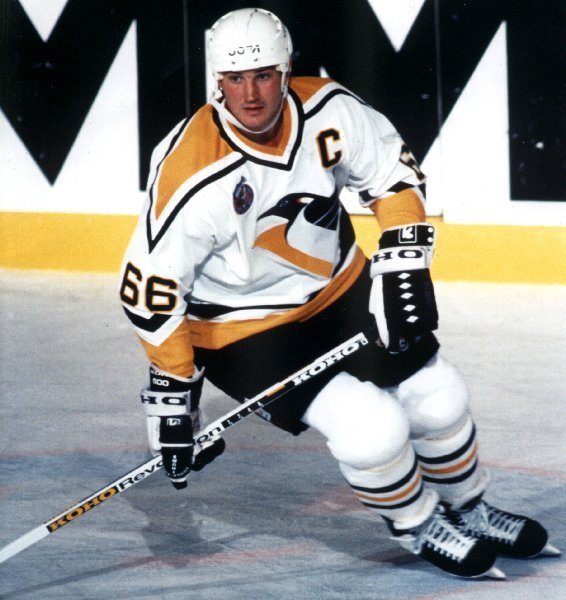
\includegraphics[height=5cm]{images/Lemieux}\\
		\centering Mario Lemieux
	\end{minipage} 
	\hfill
	\begin{minipage}[c]{.4\textwidth}
		\centering 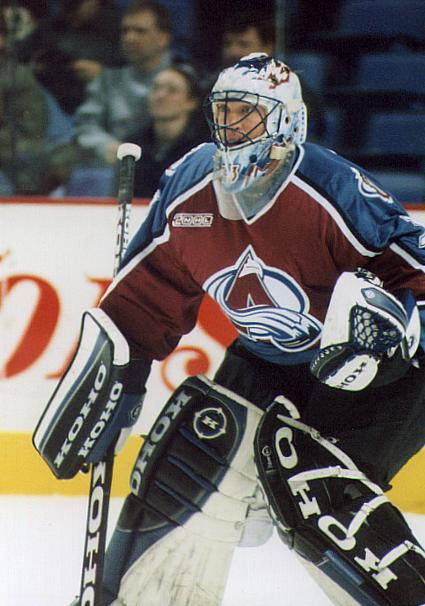
\includegraphics[height=5cm]{images/Roy}\\
		\centering Patrick Roy
	\end{minipage}
	\hfill
\end{frame}
\begin{frame}{Exemple : Quantifier l'improbable}
	\small
Soit \(E\) l'événement \textit{Les 20 meilleurs joueurs de la LNH nés dans les années 60 sont tous nés des journées différentes}. Notons qu'il y a eu \(3\times 366+7\times 365=3653\) journées durant cette période.
\pause
Décrire \(\Omega\) se fait de la manière suivante : c'est un vecteur à \num{20} composantes choisies parmi les journées des années 1960. On peut les étiqueter de 1 à 3653. La cardinalité de \(\Omega\) est donc \(\num{3653}^{20}\). \pause Un événement élémentaire appartenant à \(E\) est un vecteur dont toutes les composantes sont distinctes. On peut les énumérer de la manière suivante : il y a \num{3653} possibilités pour la première composante, \num{3652} pour la seconde, etc, jusqu'à \num{3634} pour la dernière. \pause Ainsi,
\[\P{E}=\frac{\num{3653}\times \num{3652}\times\cdots\times \num{3634}}{\num{3653}^{20}}\approx\num{0,949}=\SI{94,9}{\percent}.\]
\pause Finalement, en utilisant la propriété de complémentarité des probabilités, la probabilités qu'au moins deux joueurs parmi les 20 meilleurs nés dans les années 60 soient nés la même journée est d'environ \SI{5,1}{\percent}.
\end{frame}
\begin{frame}{Exemple : Ne tirez pas trop vite vos conclusions}
Soit \(F\) l'événement \textit{Les \num{100} meilleurs joueurs de la LNH nés dans les années \num{50}, \num{60}, \num{70}, \num{80} ou \num{90} sont tous nés des journées différentes}. \pause Notons qu'il y a eu \(\num{12}\times \num{366}+\num{38}\times \num{365}=\num{18263}\) journées durant cette période. \pause
Le raisonnement précédent nous permet de trouver que
\[\P{F}=\frac{\num{18263}\times \num{18262}\times\cdots\times \num{18164}}{\num{18263}^{100}}\approx\num{0,762}=\SI{76,2}{\percent}.\]
\pause La probabilités qu'au moins deux joueurs parmi les \num{100} meilleurs nés dans les années \num{50}, \num{60}, \num{70}, \num{80} ou \num{90} soient nés la même journée est d'environ \SI{23,8}{\percent}.
\end{frame}
\begin{frame}{La probabilité d'une union}
\pause
	\begin{props}
	\textbf{Pour deux événements :}
	
	Soit \(A\) et \(B\) deux événements. Alors
	\[\P{A\cup B}=\P{A}+\P{B}-\P{A\cap B}.\]
	
	\pause
	\medskip
	\textbf{Pour trois événements :}
	
	Soit \(A, B\) et \(C\) trois événements. Alors
		\begin{align*}
		\P{A\cup B\cup C}&=\P{A}+\P{B}+\P{C}\\
		&~~~~-\P{A\cap B}-\P{A\cap C}-\P{B\cap C}\\
		&~~~~+\P{A\cap B\cap C}.
		\end{align*}
	\end{props}
\end{frame}
\begin{frame}{Exemple : Tirer une carte}
	\begin{cadre}
	On tire une carte d'un jeu standard de 52 cartes. Quelle est la probabilité de tirer un roi ou un cœur?
	\end{cadre}
\end{frame}

\begin{frame}{La monotonicité}
\pause
	\begin{prop}{}{}
		Soit \(A\) et \(B\) deux événements tels que \(A\subseteq B\). Alors
			\[\P{A}\leq\P{B}.\]
	\end{prop}
	\pause
	On peut écrire \(B=A\cup \left(B\cap A\comp\right)\). Les événements \(A\) et \(B\cap A\comp\) étant incompatibles, on en déduit que
	\[\P{B}=\P{A}+\P{B\cap A\comp}.\]
	De là on observe que \(\P{B\cap A\comp}=\P{B}-\P{A}\). Comme la probabilité de réalisation de tout événement est \(\geq 0\), il suit que
	\[0\leq \P{B\cap A\comp}=\P{B}-\P{A}.\]
	Le résultat est finalement déduit de l'inégalité \(0\leq \P{B}-\P{A}\).
\end{frame}
\begin{frame}{Inégalité de Boole}
\pause
\begin{prop}
 Soit \(A_1,A_2,\ldots, A_n\) des événements. Alors
 \[\P{\cup_{k=1}^n A_k}\leq \sum_{k=1}^n\P{A_k}.\]
\end{prop}
\pause
	Considérons deux événements \(A\) et \(B\). \pause Nous savons que
	\[\P{A\cup B}=\P{A}+\P{B}-\P{A\cap B}.\]
	\pause On en déduit que \(\P{A\cup B}\leq \P{A}+\P{B}\).
Cette inégalité est utilisée pour majorer la probabilité de réalisation d'une union d'événements peu probables. \pause Elle est aussi valable dans le cas où on a une famille dénombrable d'événements.
\end{frame}
\begin{frame}{Exemple : Majorer avec Boole}
	\begin{cadre}
	On lance 3 dés. Majorez la probabilité d'obtenir au moins un 6.
\end{cadre}
\end{frame}
\begin{frame}{Inégalité de Bonferroni}
	\small
\pause
	\begin{prop}
 		Soit \(A_1,A_2,\ldots, A_n\) des événements. Alors
 		\[\P{\cap_{k=1}^n A_k}\geq 1-\sum_{k=1}^n\P{{A_k}\comp}.\]
	\end{prop}
	\pause
	Considérons deux événements \(A\) et \(B\). On constate que
	\[\P{A\cap B}=1-\P{A\comp\cup B\comp}.\]
	\pause
	 D'après l'inégalité de Boole, \(\P{A\comp\cup B\comp}\leq \P{A\comp}+\P{B\comp}\).\pause On en déduit que
	\[\P{A\cap B}\geq 1-\P{A\comp}-\P{B\comp}.\]
	\pause
	Cette inégalité est utilisée pour minorer la probabilité de réalisation d'une intersection d'événements probables. Elle est aussi valable dans le cas où on a une famille dénombrable d'événements.
\end{frame}
\begin{frame}{Exemple : Minorer avec Bonferroni}
	\begin{cadre}
		Minorez la probabilité que 3 lancers de dés ne donne jamais de 6.
	\end{cadre}
\end{frame}

\section{Au-delà du cas discret}
\begin{frame}[t]{Les limites de l'approche par les poids}
\pause
	On choisit un nombre réel \emph{au hasard} dans \(\Omega=\interval{0}{1}\), qui n'est pas dénombrable.
	\pause
	\begin{itemize}
		\item Tous les nombres devraient avoir le même poids \(p\).\pause
		\item Si \(p>0\), \(n>1/p\) nombres distincts formeraient un événement de probabilité \(n\cdot p>1\). \pause Il faut donc que \(p=0\).\pause
		\item Mais alors « la somme » des poids de tous les éléments de \(\Omega\) ne peut pas valoir \(1\).
	\end{itemize}
	\pause
	\begin{lumiere}
		Il faut plutôt définir directement \(\P{A}\) pour certains événements \(A\), par exemple \(\P{\interval{a}{b}}=b-a\). C'est le rôle des axiomes de Kolmogorov (module \emph{Fondements des probabilités}).
	\end{lumiere}
\end{frame}
 \begin{frame}[allowframebreaks]{Bibliographie}
 \printbibliography[heading=none]
	\vspace{0.5cm}
 \begin{rems}
 	\begin{itemize}
 		\item Ce document est rédigé avec Beamer, une classe de LaTeX.
 		\item Les diagrammes de Venn ont été réalisés en utilisant TikZ (un paquet de LaTeX).
 		\item Les images de personnes proviennent de Wikipédia.
 		\item La structure de ce document est inspirée de \cite{belisle}.
 	\end{itemize}
 \end{rems}
 	\vfill
 	\footnotesize Pour signaler une erreur dans ce document, veuillez écrire à~\href{mailto:jerome.soucy@mat.ulaval.ca}{jerome.soucy@mat.ulaval.ca}.
 \end{frame}
\end{document} 